
\section{定义及其在嵌入问题上的应用}
\label{sec:capacity-definition-embeddings}

下面，我们将引入一类特殊的\trSymplecticInvariant，它们由 I.~\trEkeland{}与%
H.~\trHofer{}在 [68, 69] 中针对 $\R^{2n}$ 的子集所发现。两人是在对%
\trConvex\trEnergySurface{}上的\trPeriodicSolution{}的搜寻中被引向这些不变量的，%
并把它们称为\trSymplecticCapacity。\trSymplecticCapacity{}的概念后来由%
H.~\trHofer{}与 E.~\trZehnder{}在 [123] 中推广到了一般的\trSymplecticManifold。%
这些不变量的存在性证明基于一个\trVariationalPrinciple；它并不直观，%
我们将把它推迟到下一章。倘若将其存在性视为理所当然，那么本章的目标毋宁说是：%
推导出某些\trSymplecticEmbedding{}的\trRigidity，此外还推导出\trMapping{}的辛性质%
在上确界\trNorm{}下的极限之下所具有的\trRigidity{}——后者将引出%
「\textbf{\trSymplecticHomeomorphism}」（symplectic homeomorphism）的概念。

\textbf{\trSymplecticCapacity{}的定义。}\quad 我们考察可能带\trBoundary、%
维数固定为 $2n$ 的\trSymplecticManifold{} $(M,\omega)$ 全体所成之类。%
一个\trSymplecticCapacity{}是一个\trMapping{} $(M,\omega)\mapsto c(M,\omega)$，%
它给每个\trSymplecticManifold{} $(M,\omega)$ 指派一个非负数或 $\infty$，%
并满足下列性质 A1--A3。

\textbf{A1. \trMonotonicity}：只要存在\trSymplecticEmbedding{}%
$\varphi:(M,\omega)\to(N,\tau)$，便有 $c(M,\omega)\leq c(N,\tau)$。

\textbf{A2. \trConformality}（conformality）：对一切 $\alpha\in\R$、$\alpha\neq0$，%
$c(M,\alpha\omega)=|\alpha|\,c(M,\omega)$。

\textbf{A3. \trNontriviality}（nontriviality）：$c(B(1),\omega_0)=\pi=c(Z(1),\omega_0)$，%
这里 $B(1)$ 是开\trUnitBall，$Z(1)$ 是\trStandard{}空间 $(\R^{2n},\omega_0)$ 中的开\trSymplectic\trCylinder。%
为方便起见，我们回顾：在\trSymplecticCoordinates{} $(x,y)\in\R^{2n}$ 之下，
\[
B(r)=\Bigl\{(x,y)\in\R^{2n}\ \Bigm|\ |x|^{2}+|y|^{2}<r^{2}\Bigr\}
\]
与
\[
Z(r)=\Bigl\{(x,y)\in\R^{2n}\ \Bigm|\ x_1^{2}+y_1^{2}<r^{2}\Bigr\}
\]
（其中 $r>0$）。人们常常发现，用下述较弱的公理 $(A3')$ 取代 (A3) 会更方便：

\textbf{A3$'$. 弱\trNontriviality}：$0<c(B(1),\omega_0)$ 且 $c(Z(1),\omega_0)<\infty$。

应当指出，公理 (A1)--(A3) 并不能唯一地确定一个\textbf{\trCapacity{}函数}%
（capacity function）。诚然，构造\trCapacity{}函数的途径很多，我们稍后即会看到。%
我们首先来阐释这一概念，并从公理 (A1)--(A3) 引出几条简单的推论。%
在二维\trSymplecticManifold（即 $n=1$）这一特殊情形，总面积的模
\[
c(M,\omega):=\Bigl|\int_{M}\omega\Bigr|
\]
便是一个\trSymplecticCapacity{}函数的例子。它与 $(\R^{2},\omega_0)$ 中的%
\trLebesgue{}\trMeasure{}相一致。与之相反，当 $n>1$ 时，\trSymplecticInvariant{}%
$\bigl(\operatorname{vol}\bigr)^{\frac{1}{n}}$ 便被公理 (A3) 排除在外，%
因为\trCylinder{}具有无穷的\trVolume。若 $\varphi:(M,\omega)\to(N,\sigma)$ 是这两个%
\trManifold{} $M$ 与 $N$ 之间的一个\trSymplecticDiffeomorphism，%
则将\trMonotonicity{}公理应用于 $\varphi$ 与 $\varphi^{-1}$ 便得出
\[
c(M,\omega)=c(N,\sigma).
\]
因此，\trCapacity{}确实是一个\trSymplecticInvariant。此外我们还注意到，%
借助\textbf{\trInclusionMapping}（inclusion mapping），对 $(M,\omega)$ 的开子集而言，\trMonotonicity
\[
U\subset V\ \Longrightarrow\ c(U)\leq c(V)
\]
成立。

为了描述 $(\R^{2n},\omega_0)$ 中的一些简单例子，我们以下述结果起步。

\begin{lemma}\label{lem:scaling}
设 $U\subset(\R^{2n},\omega_0)$ 为\trOpenSet{}且 $\lambda\neq0$，则
\[
c(\lambda U)=\lambda^{2}\,c(U).
\]
\end{lemma}

\begin{proof}
这是\trConformality{}公理的一个推论。\trDiffeomorphism
\[
\varphi:\lambda U\to U,\qquad x\mapsto\frac{1}{\lambda}\,x
\]
满足 $\varphi^{*}\bigl(\lambda^{2}\omega_0\bigr)=\lambda^{2}\,\varphi^{*}\omega_0=\omega_0$。%
因此，$\varphi:(\lambda U,\omega_0)\to(U,\lambda^{2}\omega_0)$ 是\trSymplectic{}的，%
于是恰如所断言的，$c(\lambda U,\omega_0)=c(U,\lambda^{2}\omega_0)=\lambda^{2}\,c(U,\omega_0)$。
\end{proof}

对 $\R^{2n}$ 中半径 $r>0$ 的开\trBall，我们特别得到
\begin{equation}\label{eq:ball-capacity}
c\bigl(B(r)\bigr)=r^{2}\,c\bigl(B(1)\bigr)=\pi r^{2}.
\end{equation}
由于对每个 $\varepsilon>0$ 都有 $B(r)\subset\overline{B(r)}\subset B(r+\varepsilon)$，%
借\trMonotonicity{}便得出 $c\bigl(\overline{B(r)}\bigr)=\pi r^{2}$。我们看到，%
在 $(\R^{2},\omega_0)$ 这一特殊情形，
\[
c\bigl(B(r)\bigr)\ =\ c\Bigl(\overline{B(r)}\Bigr)\ =\ \operatorname{area}\bigl(B(r)\bigr)
\]
与\trDisc{}的\trLebesgue{}\trMeasure{}相一致。借助于此可以证明：对 $\R^{2}$ 中的一大类集合，%
\trCapacity{}都与\trLebesgue{}\trMeasure{}一致，正如 K.~F.~\trSiburg{} [194]%
所观察到的那样。

\begin{proposition}\label{prop:area-capacity}
若 $D\subset\R^{2}$ 是带\trSmooth\trBoundary{}的\trCompact、\trConnected{}的%
\trDomain，则
\[
c(D,\omega_0)=\operatorname{area}(D).
\]
\end{proposition}

\begin{proof}
从 $D$ 中移去有限多条\trCompact\trCurve，便可找到一个满足 $m(D_0)=m(D)$ 的%
\textbf{\trSimplyConnected}（simply connected）\trDomain{} $D_0\subset D$；%
鉴于\textbf{\trUniformization{}定理}（uniformization theorem），它\trDiffeomorphic{}于单位\trDisc{} $B(1)\subset\R^{2}$。于是，%
存在 $\rho>0$ 与一个\trDiffeomorphism{} $\varphi:B(\rho)\to D_0$，%
它此外还满足 $m(B(\rho))=m(D_0)$。给定 $\varepsilon>0$，可以找到 $r<\rho$，%
使得 $D_1:=\varphi(B(r))\subset D_0$ 满足 $m(D_1)\geq m(D)-\varepsilon$。%
于是，由\trDacorogna-\trMoser{}定理，存在一个\trMeasurePreserving{}的%
\trDiffeomorphism{} $\psi:\overline{B(r)}\to D_1$。由于这个 $\psi$ 是\trSymplectic{}的，%
我们可以借助\trMonotonicity、\trSymplecticDiffeomorphism{}之下的\trInvariance{}%
以及\textbf{\trNormalization}（normalization）来作出估计：
\[
m(D)-\varepsilon\ \leq\ m(D_1)\ =\ m\Bigl(\overline{B(r)}\Bigr)\ =\ %
c\Bigl(\overline{B(r)}\Bigr)\ =\ c(D_1)\ \leq\ c(D).
\]
另一方面，存在\trDiffeomorphism{} $\varphi:D\to\overline{B(R)}\setminus E$，%
其中 $E$ 表示总\trMeasure{}不超过 $\varepsilon$ 的有限多个开\trDisc{}所成之集。%
适当选取 $R$，并再次借助\trDacorogna{}与\trMoser{}的定理，便可设 $\varphi$%
是\trSymplectic{}的，于是
\[
c(D)\ \leq\ c\Bigl(\overline{B(R)}\Bigr)\ =\ \pi R^{2}\ \leq\ m(D)+\varepsilon.
\]
总而言之：对每个 $\varepsilon>0$ 都有 $m(D)-\varepsilon\leq c(D)\leq m(D)+\varepsilon$，%
结论得证。
\end{proof}

显然，对 $(\R^{2n},\omega_0)$ 中每个开而\trBounded{}的集合 $U$ 都有%
$0<c(U)<\infty$，因为 $U$ 含有一个小\trBall，同时又含于一个大\trBall{}之内。%
仿照上文对 $B(r)$ 的论证，对\trSymplectic\trCylinder{}可以证明
\begin{equation}\label{eq:cylinder-capacity}
c\bigl(Z(r)\bigr)=\pi r^{2}.
\end{equation}
因此，若\trOpenSet{} $U$ 对某个 $r>0$ 满足
\[
B(r)\subset U\subset Z(r),
\]
则由\trMonotonicity{}可得 $\pi r^{2}=c\bigl(B(r)\bigr)\leq c(U)\leq%
c\bigl(Z(r)\bigr)=\pi r^{2}$，从而
\[
c(U)=\pi r^{2}.\qquad\text{（图 2.1）}
\]

\noindent\begin{minipage}{\linewidth}
\centering
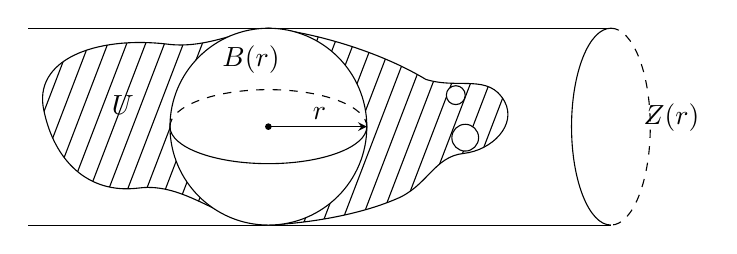
\begin{tikzpicture}[>=stealth]
  \draw (-4.55,1.25) -- (2.85,1.25);
  \draw (-4.55,-1.25) -- (2.85,-1.25);
  \def\ublob{(-4.35,0.2)
        .. controls (-4.5,0.85) and (-3.7,1.15) .. (-2.8,1.05)
        .. controls (-2.3,0.98) and (-1.9,1.22) .. (-1.5,1.25)
        .. controls (-1.1,1.22) and (-0.2,1.02) .. (0.5,0.6)
        .. controls (0.92,0.47) and (1.3,0.68) .. (1.5,0.32)
        .. controls (1.66,0.02) and (1.34,-0.3) .. (0.98,-0.34)
        .. controls (0.6,-0.38) and (0.52,-0.76) .. (0.12,-0.92)
        .. controls (-0.3,-1.1) and (-0.9,-1.22) .. (-1.5,-1.25)
        .. controls (-2.1,-1.22) and (-2.55,-0.7) .. (-3.15,-0.78)
        .. controls (-3.8,-0.86) and (-4.22,-0.42) .. (-4.35,0.2) -- cycle}
  \fill[white] \ublob;
  \begin{scope}%
    \clip \ublob;
    \foreach \x in {-5.2,-4.96,...,2.0}
      \draw (\x,-1.4) -- (\x+1.15,1.6);
  \end{scope}
  \draw \ublob;
  \fill[white] (0.88,0.40) circle (0.12);%
  \draw (0.88,0.40) circle (0.12);
  \fill[white] (1.0,-0.14) circle (0.17);
  \draw (1.0,-0.14) circle (0.17);
  \fill[white] (-1.5,0) circle (1.25);
  \draw (-1.5,0) circle (1.25);
  \draw[dashed] (-2.75,0) arc (180:0:1.25 and 0.47);%
  \draw (-2.75,0) arc (180:360:1.25 and 0.47);%
  \fill (-1.5,0) circle (1.2pt);
  \draw[->] (-1.5,0) -- (-0.25,0);%
  \node at (-0.85,0.17) {$r$};
  \node at (-1.72,0.85) {$B(r)$};
  \node at (-3.35,0.28) {$U$};
  \draw (2.85,1.25) arc (90:270:0.5 and 1.25);%
  \draw[dashed] (2.85,1.25) arc (90:-90:0.5 and 1.25);%
  \node at (3.62,0.12) {$Z(r)$};
\end{tikzpicture}

图 2.1
\end{minipage}

这表明：当 $n>1$ 时，在形状、大小、\trMeasure{}与\trTopology{}上截然不同的%
\trOpenSet{}可以具有相同的\trCapacity。回忆上一章中引入的\trEllipsoid{}%
$E\subset\R^{2n}$ 由（\trLinear{}的）\trSymplecticInvariant{}%
$r_1(E)\leq r_2(E)\leq\dots\leq r_n(E)$ 所刻画。施加一个保持诸\trCapacity{}的%
\trLinear\trSymplectic\trMapping{}之后，鉴于第 1 章中的%
\cref{thm:ellipsoid-linear-embedding}，不妨设
\[
B(r_1)\subset E\subset Z(r_1),
\]
其中 $r_1=r_1(E)$。于是我们得出结论：\trEllipsoid{} $E$ 的\trCapacity{}%
便由最小的\trLinear\trSymplecticInvariant{} $r_1(E)$ 所确定。

\begin{proposition}\label{prop:ellipsoid-capacity}
$(\R^{2n},\omega_0)$ 中\trEllipsoid{} $E$ 的\trCapacity{}由
\[
c(E)=\pi r_1(E)^{2}.
\]
给出。
\end{proposition}

我们看到，每个\trCapacity{} $c$ 都是\trEllipsoid{} $E$ 的最小\trLinear{}\trInvariant{}量%
$\pi r_1(E)^{2}$ 的一个\trContinuation；于是自然要问：$j>1$ 的那些\trLinear{}\trInvariant{}量%
$\pi r_j(E)^{2}$，能否也\trContinuation{}为\trNonlinear{}情形下的\trInvariant{}量？%
我们稍后将回到这一问题上来。%
\trSymplectic\trCylinder{}「基于」\trSymplectic{}的二维平面；它们与「基于」%
\trIsotropic{}二维平面——即\trTwoForm{} $\omega_0$ 在其上为零的那类平面——%
的\trCylinder{}截然不同，例如%
$Z_1(r)=\bigl\{(x,y)\in\R^{2n}\ \bigm|\ x_1^{2}+x_2^{2}<r^{2}\bigr\}$。我们断言：
\[
c\bigl(Z_1(r)\bigr)=+\infty,\qquad\text{对一切 } r>0.
\]
这一点很容易看出：对每个\trBall{} $B(N)$ 都存在一个\trLinear\trSymplecticEmbedding{}%
$\varphi:B(N)\to Z_1(r)$，因此 $\pi N^{2}=c\bigl(B(N)\bigr)\leq c\bigl(Z_1(r)\bigr)$。%
这对每个 $N$ 都成立，断言即得。

为了把这个例子加以推广，我们先回忆几个定义。若 $V\subset\R^{2n}$ 是一个%
\trLinear\trSubspace，则它的\trSymplecticComplement{} $V^{\perp}$ 定义为
\[
V^{\perp}=\bigl\{x\in\R^{2n}\ \bigm|\ \omega_0(v,x)=0\ \text{对一切 } v\in V\bigr\}.
\]
显然 $(V^{\perp})^{\perp}=V$，并且由于 $\omega_0$ 是\trNondegenerate{}的，%
$\dim V^{\perp}=\dim\R^{2n}-\dim V$。一个\trLinear\trSubspace{} $V$%
称为\trIsotropic{}的，若 $V\subset V^{\perp}$，也就是说%
$\omega_0(v_1,v_2)=0$\footnote{原书印作「$\omega$」，依上下文径改「$\omega_0$」。——译者注} 对一切 $v_1$ 与 $v_2\in V$ 成立。

\begin{proposition}\label{prop:cylinder-sum-subspace}
设 $\Omega\subset\R^{2n}$ 是一个\trBounded{}的非空\trOpenSet，并设 $W\subset\R^{2n}$%
是满足 $\operatorname{codim}W=2$ 的一个\trLinear\trSubspace。考虑\trCylinder{}%
$\Omega+W$，则
\[
\begin{aligned}
c(\Omega+W)&=+\infty,\qquad&&\text{若 } W^{\perp}\text{ 是\trIsotropic{}的},\\
0<c(\Omega+W)&<\infty,\qquad&&\text{若 } W^{\perp}\text{ 不是\trIsotropic{}的}.
\end{aligned}
\]
\end{proposition}

\begin{proof}
不妨设 $\Omega$ 包含原点。注意 $\dim W^{\perp}=2$。因此，在第二种情形，%
$W^{\perp}$ 是一个\trSymplectic\trSubspace，且 $\R^{2n}=W^{\perp}\oplus W$。%
于是，在 $W^{\perp}$ 中选取\trSymplecticBasis{} $(e_1,f_1)$ 之后，%
经由一个\trLinear\trSymplectic{}坐标变换便可设
\[
W=\bigl\{(x,y)\ \bigm|\ x_1=y_1=0\bigr\}.
\]
由于 $\Omega$ \trBounded，对 $z\in\Omega+W$ 存在某个 $N$ 使得 $x_1^{2}+y_1^{2}<N^{2}$；%
从而 $\Omega+W\subset B^{2}(N)\times\R^{2n-2}$，于是由%
\eqref{eq:cylinder-capacity} 得%
$c(\Omega+W)\leq c\bigl(B^{2}(N)\times\R^{2n-2}\bigr)=\pi N^{2}<\infty$。%
这就证明了第二个论断。为了证明第一个论断，可以设
\[
W=\bigl\{(x,y)\ \bigm|\ x_1=x_2=0\bigr\}.
\]
存在 $\alpha>0$，使得只要 $x_1^{2}+x_2^{2}<\alpha^{2}$ 就有%
$(x,y)\in\Omega+W$。于是每个\trBall{} $B(R)$ 都可以\trSymplectic{}地%
\trEmbedding{}到 $\Omega+W$ 之中：只需把\trLinear\trSymplectic\trMapping{}%
$\varphi$ 定义为 $\varphi(x,y)=\bigl(\varepsilon x,\ \frac{1}{\varepsilon}\,y\bigr)$；%
那么只要 $\varepsilon>0$ 取得足够小，便有 $\varphi\bigl(B(R)\bigr)\subset\Omega+W$。%
从而，由\trCapacity{}的\trMonotonicity，$c(\Omega+W)\geq c\bigl(B(R)\bigr)=\pi R^{2}$\footnote{原书印作「$\times$」，径改「$+$」。——译者注}。%
这对每个 $R>0$ 都成立，故如所断言的，$c(\Omega+W)=+\infty$。
\end{proof}

鉴于\trMonotonicity，这些\trSymplecticInvariant{} $c(M,\omega)$%
尤其构成\trSymplecticEmbedding{}的\trObstruction。诸公理的一个直接推论，%
便是\trGromov{}那著名的\trSqueezingTheorem{} [107]——正是它催生了\trCapacity{}的概念。

\begin{theorem}[\trGromov\trSqueezingTheorem]\label{thm:capacity-squeezing}
存在\trSymplecticEmbedding{} $\varphi:B(r)\to Z(R)$ 当且仅当 $R\geq r$。
\end{theorem}

\begin{proof}
若 $\varphi$ 是一个\trSymplecticEmbedding，则利用\trCapacity{}的%
\trMonotonicity，并结合 \eqref{eq:ball-capacity} 与%
\eqref{eq:cylinder-capacity}，便得到
\[
\pi r^{2}=c\bigl(B(r)\bigr)\leq c\bigl(Z(R)\bigr)=\pi R^{2},
\]
定理即证。
\end{proof}

下面这个结果同样显示了\trVolumePreserving{}与\trSymplecticDiffeomorphism{}之间的差异。我们在%
$(\R^{4},\omega_0)$ 中取\trSymplecticCoordinates{} $(x_1,y_1,x_2,y_2)$，%
考察辛的开二维\trBall{} $B(r_1)$ 与 $B(r_2)$ 之乘积 $B(r_1)\times B(r_2)$。%
经由一个\trLinear\trSymplectic\trMapping，可以设 $r_1\leq r_2$。

\begin{proposition}\label{prop:product-two-balls}
存在\trSymplecticDiffeomorphism{} $\varphi:B(r_1)\times B(r_2)\to%
B(s_1)\times B(s_2)$ 当且仅当 $r_1=s_1$ 且 $r_2=s_2$。
\end{proposition}

注意，与之相对照，对每个 $r>0$ 都存在一个\trLinear\trVolumePreserving\trDiffeomorphism{}%
$\psi:B(1)\times B(1)\to B(r)\times B\bigl(\frac{1}{r}\bigr)$。%
当 $r\to0$ 时，显然有
\[
\left\{
\begin{aligned}
c\Bigl(B(r)\times B\bigl(\tfrac{1}{r}\bigr)\Bigr)\quad&\longrightarrow\quad 0\\
\operatorname{vol}\Bigl(B(r)\times B\bigl(\tfrac{1}{r}\bigr)\Bigr)\quad&=\quad\text{const.}
\end{aligned}
\right.
\]

\begin{proof}
由于 $r_1\leq r_2$，我们可以利用这个\trDiffeomorphism{} $\varphi$ 来定义%
\trSymplecticEmbedding
\[
B^{4}(r_1)\longrightarrow B(r_1)\times B(r_2)\xrightarrow{\ \varphi\ }%
B(s_1)\times B(s_2)\longrightarrow B(s_1)\times\R^{2}=Z(s_1),
\]
其中第一个与最后一个\trMapping{}均为\trInclusionMapping。由 $c$ 的\trMonotonicity{}得出%
$s_1\geq r_1$。对 $\varphi^{-1}$ 应用同一论证，得 $r_1\geq s_1$，%
于是 $r_1=s_1$。此时 $\varphi$ 是\trVolumePreserving{}的，故 $r_1r_2=s_1s_2$，结论得证。
\end{proof}

显然，倘若假定 $\varphi$ 到\trBoundary{}处都是\trSmooth{}的，%
那么关于半径的这些条件便可以由\trAction{}在\trSymplecticDiffeomorphism{}%
之下的\trInvariance{}直接读出：$|A(\partial B(r_j))|=\pi r_j^{2}$。%
人们或许会预期，与\cref{prop:product-two-balls}中相同的\trRigidity{}%
在 $\R^{2n}$ 中 $n$ 个辛的开二维\trBall{}之乘积的一般情形下也成立。情形确实如此，%
但它并不能单凭\trCapacity{}函数 $c$ 推出。事实上，[52] 中给出的证明相当精微，%
它用到了由 A.~\trFloer{}与 H.~\trHofer{}在 [90] 中发展的%
\textbf{\trSymplectic\trHomology}（symplectic homology）理论，%
另见 K.~\trCieliebak、A.~\trFloer、H.~\trHofer{}与 K.~\trWysocki{} [52]。%
最后，上一章中提到的关于\trEllipsoid{}之\trSymplecticEmbedding{}的那些%
限制条件，可由\cref{prop:ellipsoid-capacity}立即推出。

\begin{proposition}\label{prop:ellipsoid-r1-embedding}
设 $E$ 与 $F$ 是 $(\R^{2n},\omega_0)$ 中的两个\trEllipsoid。%
若 $\varphi:E\to F$ 是一个\trSymplecticEmbedding，则
\[
r_1(E)\leq r_1(F).
\]
\end{proposition}

一个\trCapacity{}函数的存在性，使得构造出许多别的\trCapacity{}函数成为可能。

作为说明，我们将证明：出现在\trGromov{}的工作 [107] 之中、并已在引言%
中解释过的\trGromovWidth{} $D(M,\omega)$ 是一个满足 (A1)--(A3) 的%
\trSymplecticCapacity。回忆由\trDarboux{}定理，当 $\varepsilon$ 充分小时%
总有\trSymplecticEmbedding{} $\varphi:(B(\varepsilon),\omega_0)\to(M,\omega)$，%
并定义
\[
D(M,\omega)=\sup\Bigl\{\pi r^{2}\ \Bigm|\ \text{存在\trSymplecticEmbedding{}}\
\varphi:\bigl(B(r),\omega_0\bigr)\to(M,\omega)\Bigr\}.
\]

\begin{theorem}\label{thm:gromov-width-capacity}
\trGromovWidth{} $D(M,\omega)$ 是一个\trSymplecticCapacity。此外，
\[
D(M,\omega)\leq c(M,\omega)
\]
对每个\trCapacity{}函数 $c$ 都成立。
\end{theorem}

由于\trCompact\trSymplecticManifold{} $(M,\omega)$ 具有有限的\trVolume，%
我们得出：对\trCompact\trManifold{}有 $D(M,\omega)<\infty$。%
这与下一章中构造的特殊\trCapacity{}函数 $c_{0}$ 恰成对照——%
后者对某些\trCompact\trManifold{}可以取到值 $\infty$。

\begin{proof}
\trMonotonicity{}公理 (A1) 已经在引言中验证过了。为了验证\trConformality{}公理%
(A2)，即对 $\alpha\neq0$ 有 $D(M,\alpha\omega)=|\alpha|\,D(M,\omega)$，%
只需证明：对每个\trSymplecticEmbedding
\[
\varphi:\bigl(B(r),\omega_0\bigr)\to(M,\alpha\omega),
\]
都对应有一个\trSymplecticEmbedding
\[
\hat{\varphi}:\Bigl(B\bigl(\tfrac{r}{\sqrt{|\alpha|}}\bigr),\omega_0\Bigr)%
\longrightarrow(M,\omega),
\]
反之亦然；于是按 $D$ 的定义便得出 $D(M,\alpha\omega)=|\alpha|\,D(M,\omega)$。%
设 $\varphi:(B(r),\omega_0)\to(M,\alpha\omega)$ 是一个\trSymplecticEmbedding，%
则 $\varphi^{*}(\alpha\omega)=\omega_0$，于是
\[
\varphi^{*}\omega=\frac{1}{\alpha}\,\omega_0.
\]
简记 $\rho=\frac{r}{\sqrt{|\alpha|}}$，我们定义\trDiffeomorphism{}%
$\psi:B(\rho)\to B(r)$ 为 $\psi(x)=\sqrt{|\alpha|}\cdot x$，并得到
\[
\psi^{*}\Bigl(\frac{1}{\alpha}\,\omega_0\Bigr)=\frac{|\alpha|}{\alpha}\,\omega_0.
\]
这样，当 $\alpha>0$ 时，\trMapping{} $\hat{\varphi}=\varphi\circ\psi:(B(\rho),\omega_0)\to(M,\omega)$%
便是所想要的\trSymplecticEmbedding。当 $\alpha<0$ 时，我们先引入%
\trSymplecticDiffeomorphism{} $\psi_0:(B(\rho),\omega_0)\to(B(\rho),-\omega_0)$，%
其定义为 $\psi_0(u,v)=(-u,v)$ 对一切 $(u,v)\in\R^{2n}$ 成立，%
然后便得到所要的\trEmbedding{}%
$\hat{\varphi}=\varphi\circ\psi\circ\psi_0:(B(\rho),\omega_0)\to(M,\omega)$。

$D\bigl(B(r),\omega_0\bigr)=\pi r^{2}$ 的验证是容易的。%
若 $\varphi:B(R)\to B(r)$ 是一个\trSymplecticEmbedding，%
则由于 $\varphi$ \trVolumePreserving，我们得出 $R\leq r$。另一方面，%
\trIdentityMap{}给出一个\trSymplecticEmbedding{} $B(r)\to B(r)$，故断言得证。%
又，由\trGromov{}的\trSqueezingTheorem，存在\trSymplecticEmbedding{}%
$\varphi:B(R)\to Z(r)$ 当且仅当 $r\geq R$，于是%
$D\bigl(Z(r),\omega_0\bigr)=\pi r^{2}$，即\trGromovWidth{}也满足\trNontriviality{}公理%
(A3)。为了证明定理的最后一条论断，设 $c(M,\omega)$ 为任意一个\trCapacity。%
若 $\varphi:B(r)\to M$ 是一个\trSymplecticEmbedding，%
则由\trMonotonicity{}得 $\pi r^{2}=c\bigl(B(r),\omega_0\bigr)\leq c(M,\omega)$。%
取上确界，便得 $D(M,\omega)\leq c(M,\omega)$，恰如定理中断言的那样。
\end{proof}

对一个给定的\trCapacity{} $c$，可以联系上它的\textbf{\trInnerCapacity}%
（inner capacity）$\check{c}$，其定义如下：
\[
\check{c}(M,\omega)=\sup\bigl\{c(U,\omega)\ \bigm|\ U\subset M\ %
\text{为\trOpenSet{}且}\ \overline{U}\subset M\setminus\partial M\bigr\}.
\]

相应地，我们引入如下\textbf{\trhDefinition}：一个\trCapacity{} $c$%
称为在 $M$ 处具有\textbf{\trInnerRegularity}（inner regularity），若
\[
\check{c}(M,\omega)=c(M,\omega).
\]

\begin{proposition}\label{prop:inner-capacity}
函数 $\check{c}$ 是一个具有\trInnerRegularity{}的\trCapacity，并且满足 $\check{c}\leq c$。%
此外，若 $d$ 是任何一个具有\trInnerRegularity{}且满足 $d\leq c$ 的\trCapacity，%
则 $d\leq\check{c}$。
\end{proposition}

\begin{proof}
从诸定义与\trCapacity{}的公理出发，证明便可立得。设例如 $d$ 是一个满足%
$d\leq c$ 且具有\trInnerRegularity{}的\trSymplecticCapacity。于是
\[
\begin{aligned}
\check{d}(M)\ &=\ \sup\bigl\{d(U)\ \bigm|\ U\subset M,\ %
\overline{U}\subset M\setminus\partial M\bigr\}\\
&\leq\ \sup\bigl\{c(U)\ \bigm|\ U\subset M,\ %
\overline{U}\subset M\setminus\partial M\bigr\}\\
&=\ \check{c}(M),
\end{aligned}
\]
恰如所断言的。
\end{proof}

由于\trGromovWidth{}是最小的\trCapacity，它具有\trInnerRegularity；%
具有这一性质的另一个例子是第 3 章中引入的\trCapacity{} $c_{0}$。%
如果我们考察一个给定的\trManifold{}的子集，那么还可以定义%
（相对于该\trManifold{}而言的）\textbf{\trOuterRegularity}（outer regularity）的概念。%
一个集合的\textbf{\trOuterCapacity}（outer capacity）定义为：%
对该集合之\trClosure{}的一切开\trNeighborhood{}的\trCapacity{}取下确界。%
这一概念我们将在下一节中再作讨论。
